\section{Deletions to additions}

For both granularities (per data point and per day), there is a trend of decreasing frequency of ratios with the increase of deletions relative to additions \ref{fig:del_to_add}. There are two apparent exceptions from this tendency. The days with a slightly higher number of deletions to additions are much more frequent than in the case of data points. Apart from that, quite common are occurrences where the number of deletions is much higher than additions.

\begin{figure}[htbp]
  \centering
  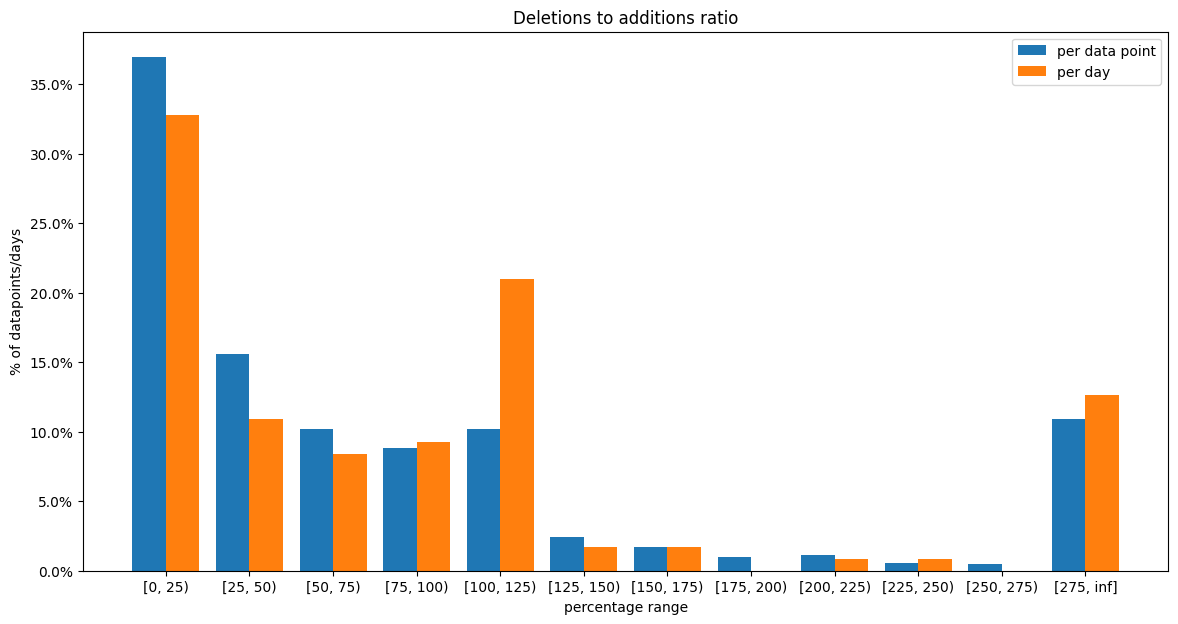
\includegraphics[scale=0.5]{chapters/results/graphics/del-to-add.png}
  \caption{Deletions to additions with regards to data points and days}
  \label{fig:del_to_add}
\end{figure}

There are no particular differences between Python and JS/TS developers with regards to the regarded ratio. One thing that is visible is the higher occurrence of the data points with lower ratio (i.e. more additions) in the case of Python comparing to JS/TS.

\begin{figure}[htbp]
  \centering
  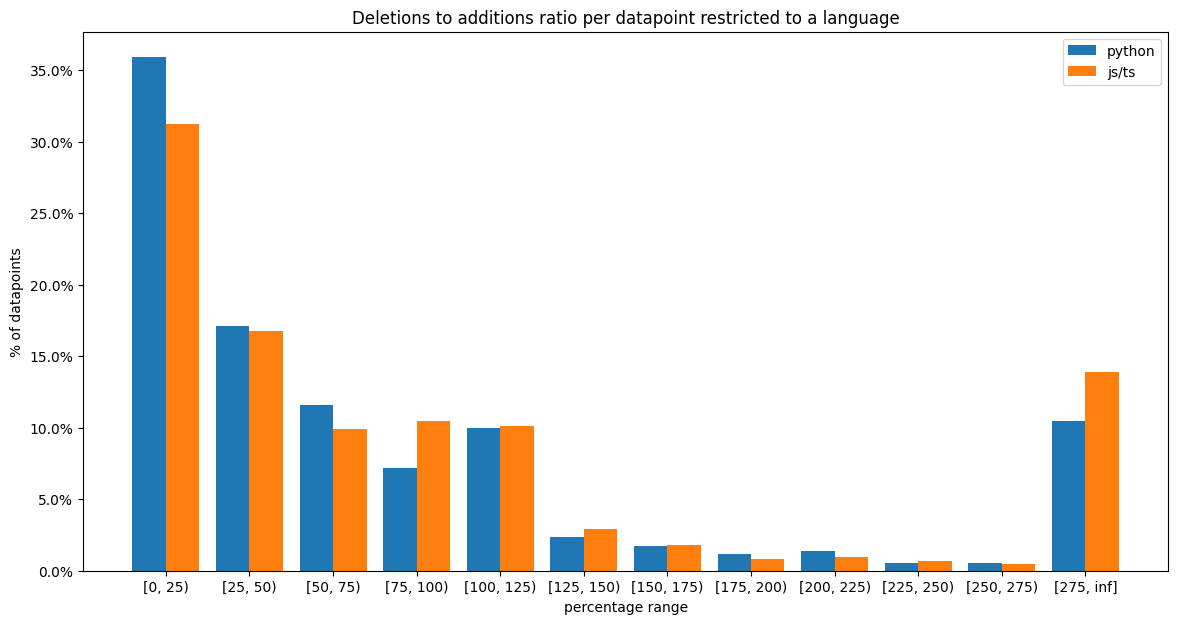
\includegraphics[scale=0.5]{chapters/results/graphics/del-to-add-langs.png}
  \caption{Deletions to additions restricted to a language}
  \label{fig:del_to_add_langs}
\end{figure}
